\chapter{Magnetostatic field calculation 3D}
To compute the total magnetostatic energy, the ferromagnetic systems can be discretized as three-dimensional cubes.\\
  
\begin{figure}[h]
	\centering
	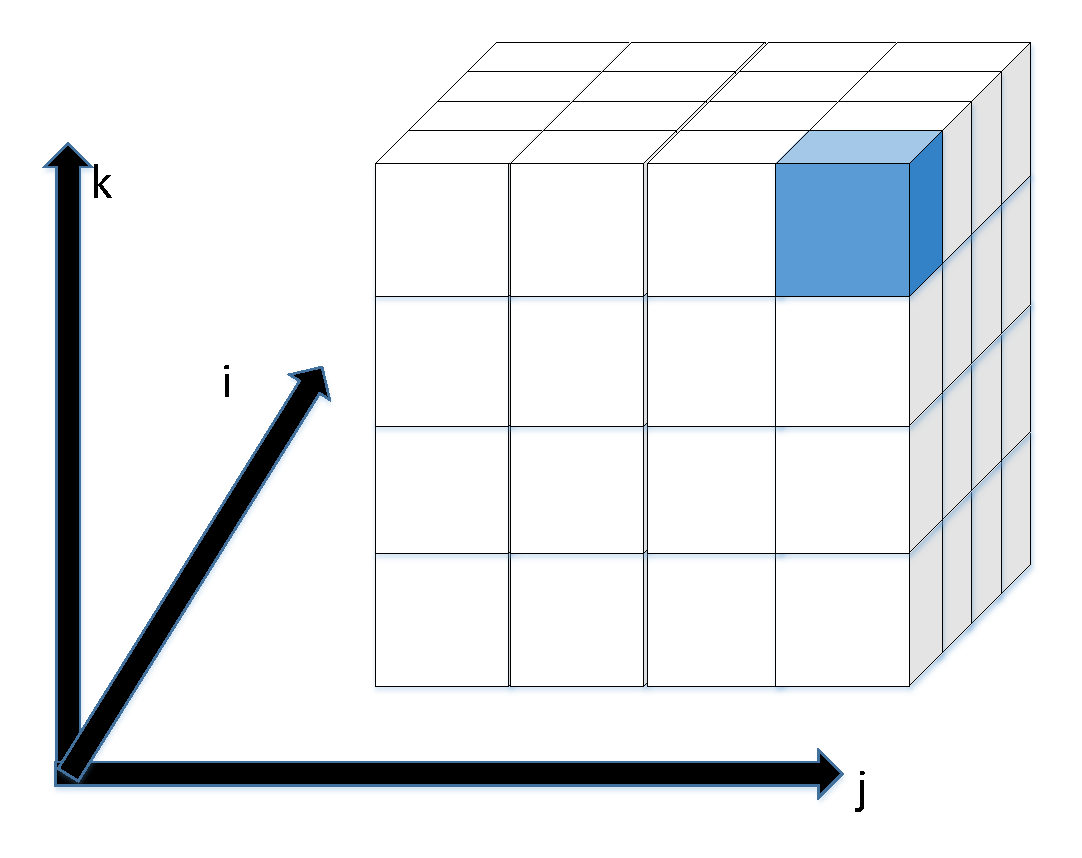
\includegraphics[width=0.7\textwidth]{imm/3d/cube.pdf}  
	\caption{The selected cell is supposed to sum all the magnetostatic field contributions between it and all the other cells}
	\label{fig:cube}
\end{figure}
  The following is the implementation of an algorithm shown in the paper \cite{3dtesi}, related to the evaluation of the contribution of the magnetostatic field to the total energy of a system. \\In general, the magnetostatic field is connected to the magnetization $ [\overrightarrow{M}] $ through the magnetizing tensor [\textbf{TG}].
  
  
  The evaluation of the magnetostatic field of a given cell requires the summation on all cells of the mesh due to the the long range of the dipole interaction.
  
  \begin{equation} \label{3d_formula}
  \overrightarrow{H}(ijk)=-M_{s}\sum\limits_{i'=1}^{N_{x}} \sum\limits_{j'=1}^{N_{y}}\sum\limits_{k'=1}^{N_{z}}\begin{bmatrix}
  TG_{xx} & TG_{xy} & TG_{xz}\\
  TG_{yx} & TG_{yy}& TG_{yz}    	\\
  TG_{zx}&TG_{zy} & TG_{zz}  
  \end{bmatrix}_{(i-i',j-j',k-k')}\begin{bmatrix}
  m_{x}\\
  m_{y}\\
  m_{z}\end{bmatrix}_{(i',j',k')}
  \end{equation}
  
  \section{Product TG and M}
  Each cell $ (i'j'k') $ has a finite state machine that evaluates the magnetostatic field contribution between the cell \textit{ijk} and the cell \textit{i'j'k'}.
  \begin{center}
  		$ \overrightarrow{h}(i-i',j-j',k-k')= \begin{bmatrix}
  	TG_{xx} & TG_{xy} & TG_{xz}\\
  	TG_{yx} & TG_{yy}& TG_{yz}    	\\
  	TG_{zx}&TG_{zy} & TG_{zz}  
  	\end{bmatrix}_{(i-i',j-j',k-k')}\begin{bmatrix}
  	m_{x}\\
  	m_{y}\\
  	m_{z}\end{bmatrix}_{(i',j',k')}$
  \end{center}.
  
  The matrix \textbf{TG}$ _{(i-i',j-j',k-k')} $ is the magnetizing tensor between the 2 cells, while $ \overrightarrow{M}_{(i',j'k')} $ is the magnetization of the cell $ i',j',k'$.\\\\
  The FSM is composed by the following states:
  \begin{itemize}
  	 \item \textbf{READ\_MX}: save $ m_x $ value
  	 \item \textbf{READ\_MY}: save $ m_y $ value
  	 \item \textbf{READ\_MZ}: save $ m_z $ value
  	 \item \textbf{READ\_TGxx}: read $ TG_{xx} $ value and computing $ op1= TG_{xx}\cdot m_x$
  	 \item \textbf{READ\_TGxy}: read $ TG_{xy} $ value and computing $ op2= TG_{xy}\cdot m_y$
  	 \item \textbf{READ\_TGxz}: read $ TG_{xz} $ value and computing $ h_x= TG_{xz}\cdot m_z +op1+op2$.
  	 \item \textbf{READ\_TGyx}:read $ TG_{yx} $ value and computing $ op1= TG_{yx}\cdot m_x$
  	 \item \textbf{READ\_TGyy}:read $ TG_{yy} $ value and computing $ op2= TG_{yy}\cdot m_y$
  	 \item \textbf{READ\_TGyz}: read $ TG_{yz} $ value and computing $ h_y= TG_{yz}\cdot m_z +op1+op2$
  	 \item \textbf{READ\_TGzx}:read $ TG_{zx} $ value and computing $ op1= TG_{zx}\cdot m_x$
  	 \item \textbf{READ\_TGzy}:read $ TG_{zy} $ value and computing $ op2= TG_{zy}\cdot m_y$
  	 \item \textbf{READ\_TGzz}: read $ TG_{zz} $ value and computing $ h_z= TG_{zz}\cdot m_z +op1+op2$
  \end{itemize}
   
     \section{Logic Plane}
     This component groups all the cells in a given plane, and enables the computation of the magnetostatic field contributions between the cell \textit{ijk} and all the cells in a given plane (i.e. $ k $ is fixed).
     \begin{center}
     	$ \overrightarrow{h}(i-i',j-j',k-k^*)$\quad \quad $ \forall i'<N_x,$\quad $ j'<N_y,$ \qquad $ k=k^* $\\
     	   \end{center}
     	   which can be also seen as	$ \overrightarrow{h}(i-i',j-j',k-k^*)$ can be computed as
     	      \begin{center}
     	$ \begin{bmatrix}
     	TG_{xx} & TG_{xy} & TG_{xz}\\
     	TG_{yx} & TG_{yy}& TG_{yz}    	\\
     	TG_{zx}&TG_{zy} & TG_{zz}  
     	\end{bmatrix}_{(i-i',j-j',k-k^*)}\begin{bmatrix}
     	m_{x}\\
     	m_{y}\\
     	m_{z}\end{bmatrix}_{(i',j',k^*)} $ \quad \quad $ \forall i'<N_x,$ \quad $ j'<N_y,$ 
     \end{center}
          All this computation can be done in parallel. 
          
          \begin{figure}[h]
          	\centering
          	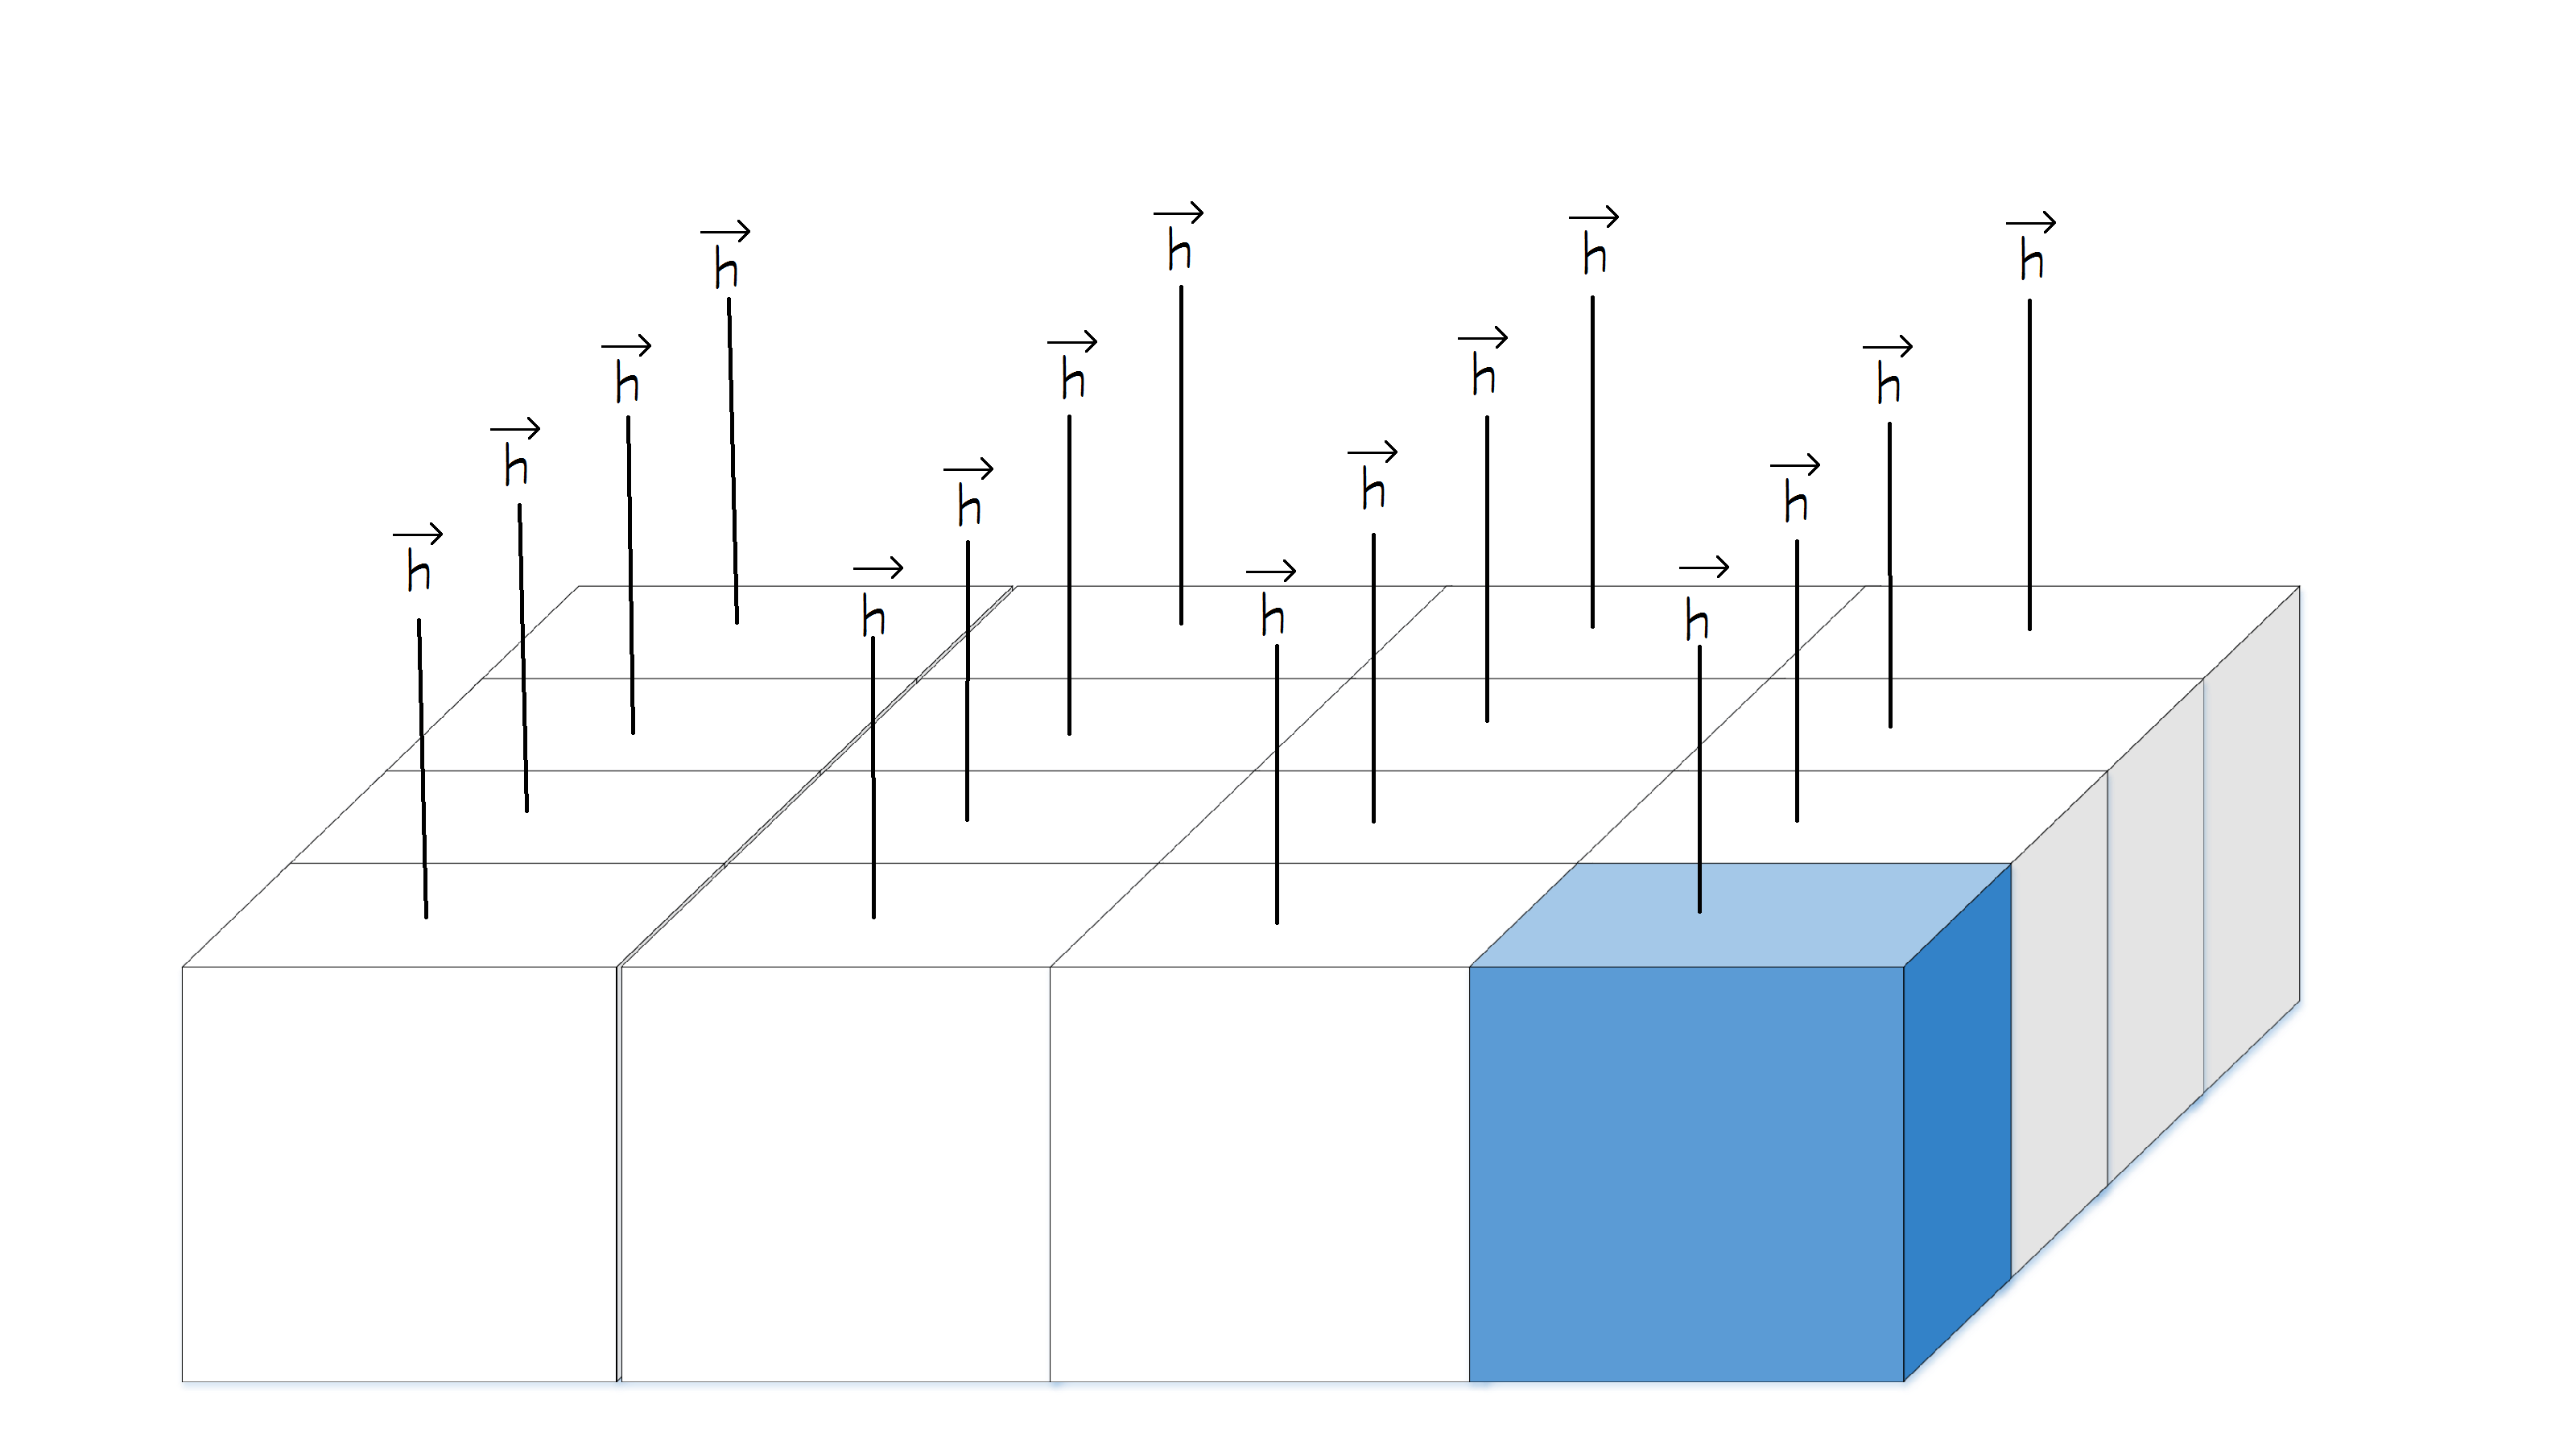
\includegraphics[width=0.9\textwidth]{imm/3d/logic_plane1.png}  
          	\caption{Magnetostatic field of each cell in a given plane}
          	\label{fig:logic_ plane}
          \end{figure}
    \section{Sum all}
    The \textit{sum\_all} is a component that given a fixed $ k^* $ (i.e. a given plane) evaluates the magnetostatic field of all cells in a fixed plane.
    The input is given by the \textit{logic plane}, as shown in the fig. \ref{fig:logic_ plane}.
    \begin{center}
    	$ \sum\limits_{i'=1}^{N_{x}} \sum\limits_{j'=1}^{N_{y}}\begin{bmatrix}
    	TG_{xx} & TG_{xy} & TG_{xz}\\
    	TG_{yx} & TG_{yy}& TG_{yz}    	\\
    	TG_{zx}&TG_{zy} & TG_{zz}  
    	\end{bmatrix}_{(i-i',j-j',k-k^*)}\begin{bmatrix}
    	m_{x}\\
    	m_{y}\\
    	m_{z}\end{bmatrix}_{(i',j',k^*)} $
    \end{center}
    By looking to the formula \ref{3d_formula}, we have to evaluate the sum for each plane, so we store this sum and wait for the next plane to be computed and added to the previous sum.\\
    Of course when we reach the $ k^{th} $ plane, we stop the sum and we set a signal to tell that the calculation is finished.\\
    Overall, this component perform the following computation\\
    \begin{center}
    	$ \sum\limits_{k'=1}^{N_{z}}\begin{pmatrix}
    	\sum\limits_{i'=1}^{N_{x}} \sum\limits_{j'=1}^{N_{y}}\begin{bmatrix}
    	TG_{xx} & TG_{xy} & TG_{xz}\\
    	TG_{yx} & TG_{yy}& TG_{yz}    	\\
    	TG_{zx}&TG_{zy} & TG_{zz}  
    	\end{bmatrix}_{(i-i',j-j',k-k')}\begin{bmatrix}
    	m_{x}\\
    	m_{y}\\
    	m_{z}\end{bmatrix}_{(i',j',k')}
    	\end{pmatrix} $
    \end{center}
    \bigskip
\section{Simulation and Test}
I wrote a testbench to check the correct behaviour of this architecture.
\subsection{Testbench of the cell}
First we check that the component \textit{cell} is working according to the specifications.
We can distinguish the 4 main phase of this test as shown in fig. \ref{fig:tb_cell_phases}.
  \begin{figure}[h]
  	\centering
  	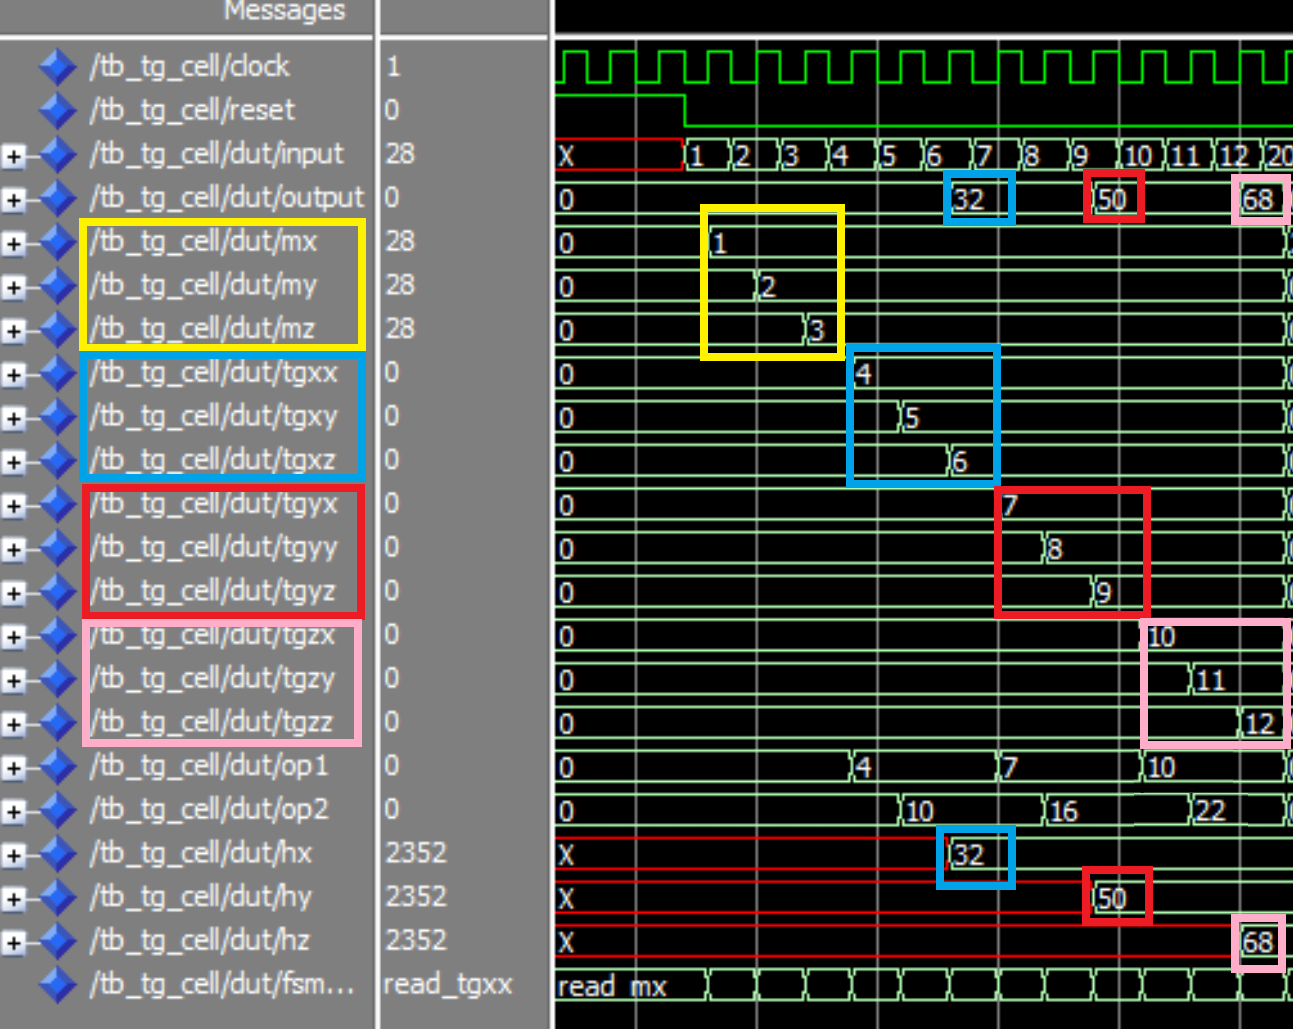
\includegraphics[width=\textwidth]{imm/3d/tb_cell_phases.png}  
  	\caption{The phases of a single cell}
  	\label{fig:tb_cell_phases}
  \end{figure}
The 4 phases are
\begin{enumerate}
	\item \textbf{Reading the magnetization}: here we read the magnetization in the 3 direction. 
	This phase is highlighted in yellow in the figure.\\ \ref{fig:tb_cell_phases}.
	$ m_x=1 $, $ m_y=2 $, $ m_z=3 $, 
	\item \textbf{Reading the magnetization x-axis}: Reading the magnetizing tensor contributions between 2 cells. Right now we look only to the contributions along the x-axis with the x-axis, y-axis, z-axis.\\In the meantime we can evaluate the magnetostatic field $ h_{x} $.
	This phase is highlighted in blue in the figure.\\
	$ tg_{xx}=4 $, $ tg_{xy}=5 $, $ tg_{xz}=6 $\\
	$ op1=m_x \cdot tg_{xx}=4 $\\
	$ op2=m_y \cdot tg_{xy}=10 $\\
	$ h_x=op1+op2+m_z \cdot tg_{xz}=32$\\
	$ output=h_x=32$
	\item \textbf{Reading the magnetization y-axis}: Similarly as the previous phase, we look only to the magnetizing tensor contributions along the y-axis with the x-axis, y-axis, z-axis.\\In the meantime we can evaluate the magnetostatic field $ h_{y} $.
	This phase is highlighted in red in the figure.\\
	$ tg_{yx}=7 $, $ tg_{yy}=8 $, $ tg_{yz}=9 $\\
	$ op1=m_x \cdot tg_{yx}=7 $\\
	$ op2=m_y \cdot tg_{yy}=16 $\\
	$ h_x=op1+op2+m_z \cdot tg_{yz}=50$\\
	$ output=h_x=50$
	\item \textbf{Reading the magnetization z-axis}: Similarly as the previous phase.
	This phase is highlighted in pink in the figure.\\
	$ tg_{yx}=10 $, $ tg_{yy}=11 $, $ tg_{yz}=12 $\\
	$ op1=m_x \cdot tg_{yx}=10 $\\
	$ op2=m_y \cdot tg_{yy}=22 $\\
	$ h_x=op1+op2+m_z \cdot tg_{yz}=68$\\
	$ output=h_x=68$
\end{enumerate}
After these 4 phases, the cell starts again from phase 1 as shown in fig. \ref{fig:tb_cell}.
\begin{figure}[h]
	\centering
	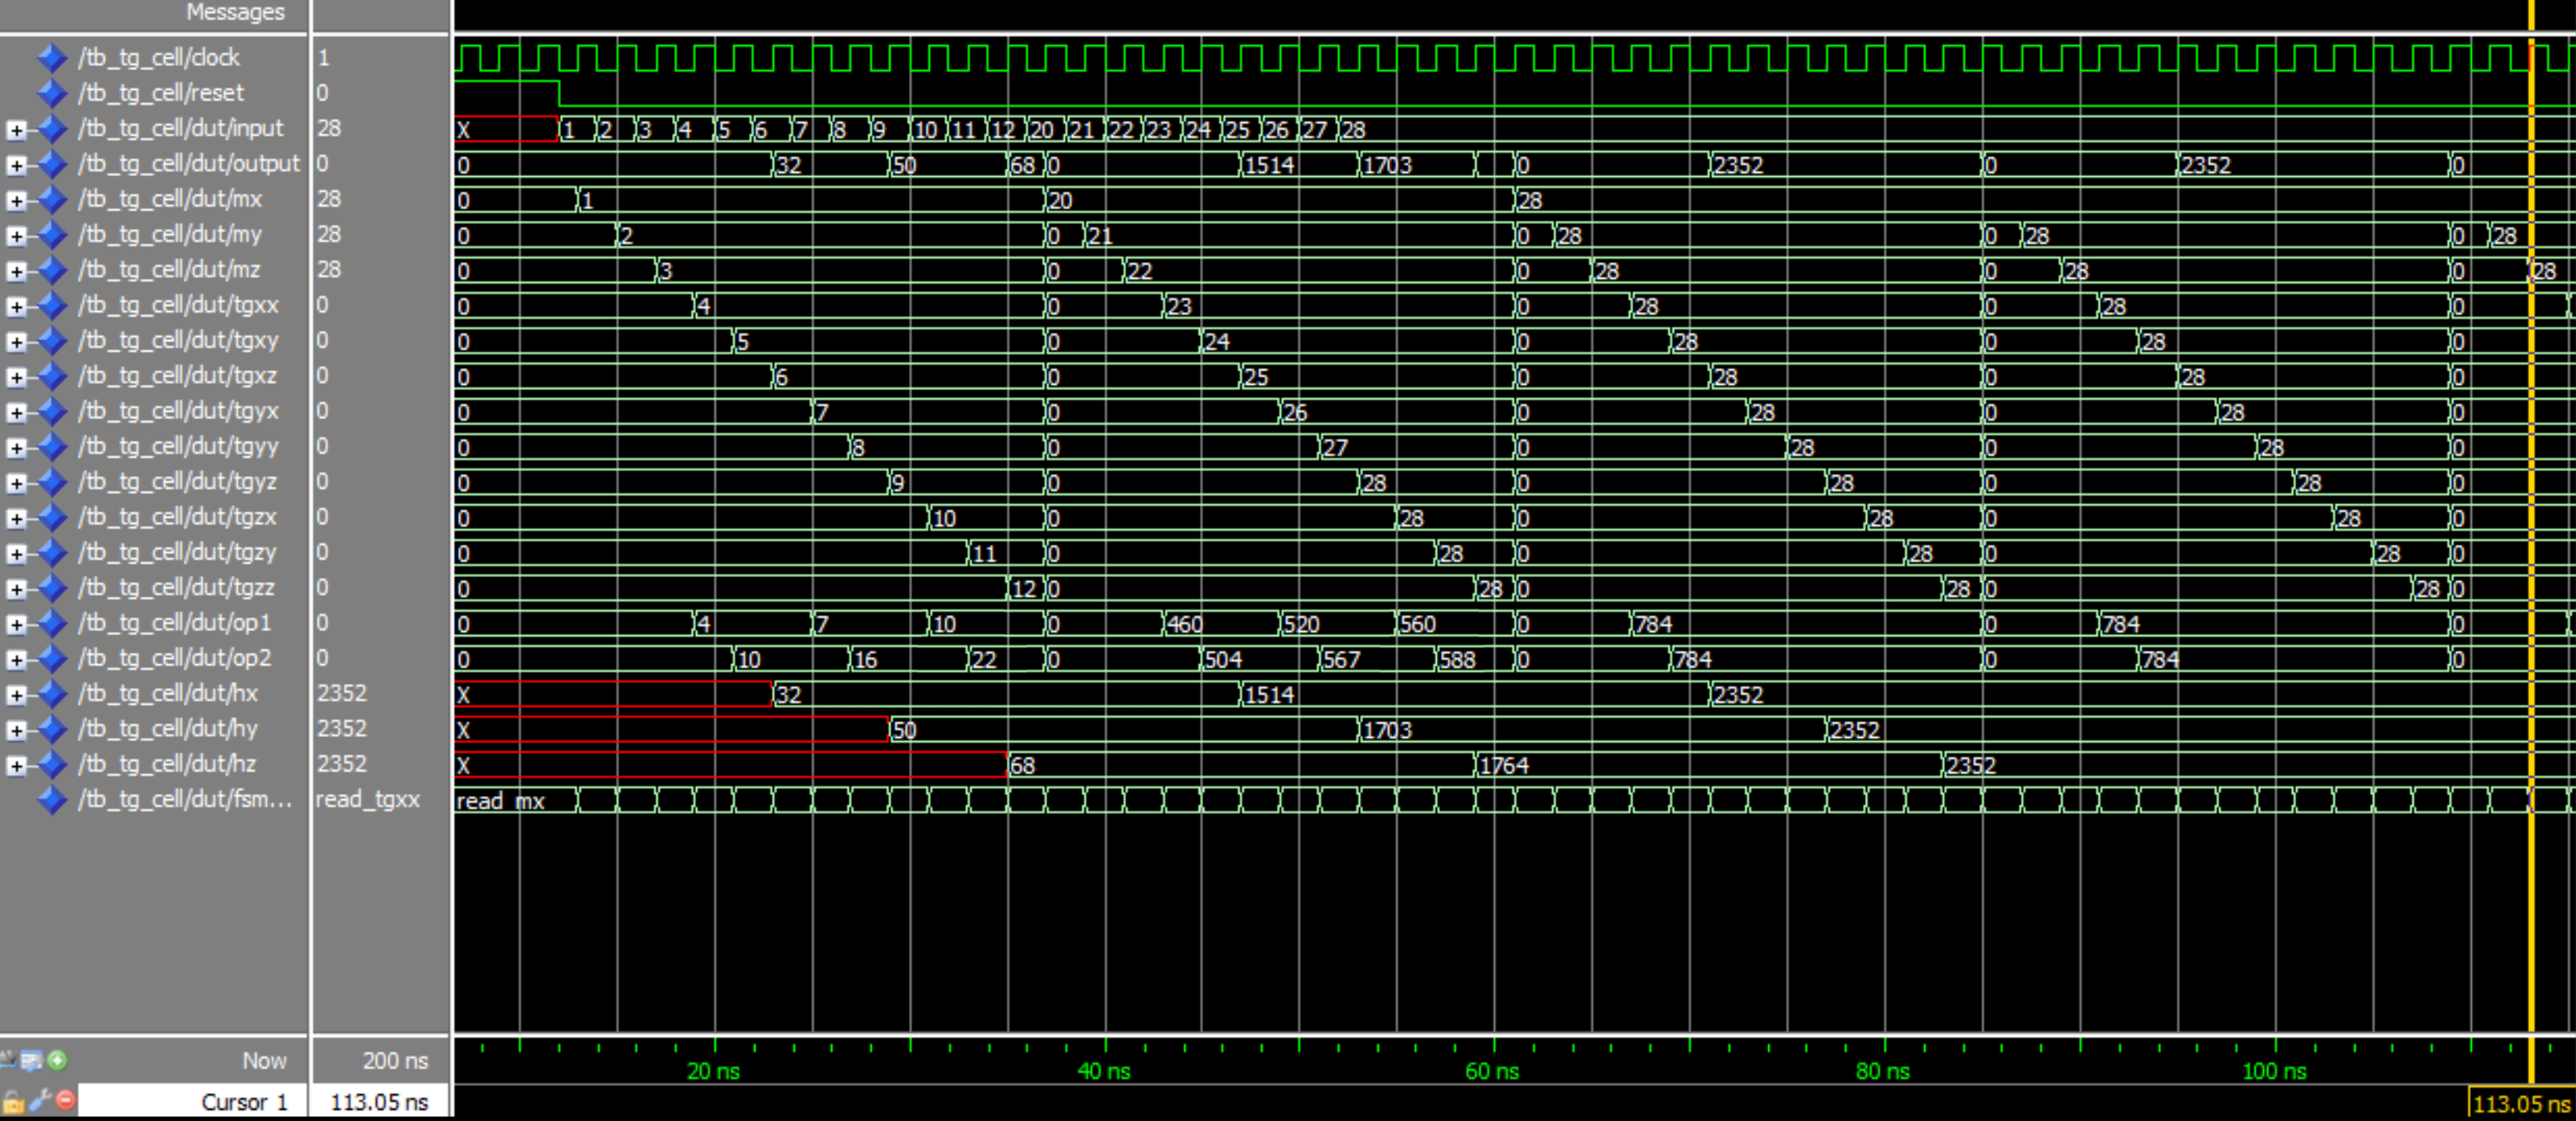
\includegraphics[width=\textwidth]{imm/3d/tb_cell.png}  
	\caption{Testbench of a single cell}
	\label{fig:tb_cell}
\end{figure}
\subsection{Testbench of the Top entity}
After testing the \textit{cell} components, we integrate them (\textit{logic\_plane}) with the \textit{sum\_all} accumulator.\\
The \textit{logic\_plane} and the \textit{sum\_all} components have to be synchronized, so a delay is needed (i.e. the logic plane evaluate the magnetostatic field of a plane and then the accumulator is ready to sum).
\clearpage
\newpage 
\section{Characteristics of Magnetostatic field calculation 3D}
\vspace{10pt}
{\large \textbf{PROCESSING ELEMENTS}}\vspace{10pt}\\
\begin{tabular}{ p{0.2cm} p{14.5cm}}
	
	&\textbf{1- Which kind of Processing element?}\\
	&	Adder, multiplier\vspace{7pt}\\
	&	\textbf{2- Functionality}\\
	&	Addition, multiplications (Evaluatin the multiplication between matrix and vectors. Another function is the accumulator.).\vspace{7pt}\\
	&	\textbf{3- Complexity}\\
	&	\begin{tabular}{ p{0.2cm} p{1.2cm}  p{13cm}}
		
		& Area: &$ i\cdot j $ cells\\
		& & one accumulator\\
		& Time: & (12 clock cycles)$\cdot k$\vspace{3pt}\\
		
		
	\end{tabular}\vspace{7pt}\\
	&	\textbf{4- Parallelism}\\
	&	Each cell can evaluate their magnetostatic contributions.\vspace{7pt}\\
	&	\textbf{5-Reconfigurability}\\
	&	No\vspace{7pt}\\
	&	\textbf{6- Programmability}\\
	&	No\vspace{7pt}\\
	&	\textbf{7- Need a dedicated memory?}\\
	&	Yes, to store the magnetization values ($m_x, m_y, m_z$)\vspace{7pt}\\
	&\textbf{8- Relationship with I/O}\\
	&	INPUT: values of the magnetization values, magnetizing tensor of each cells.\\
	&	OUTPUT: result of the magnetostatic field. algorithm\end{tabular}\vspace{74pt}\\
\newpage{\large \textbf{\qquad }}\vspace{10pt}\\
{\large \textbf{MEMORY ELEMENTS}}\vspace{10pt}\\\begin{tabular}{ p{0.2cm} p{14.5cm}}
	&\textbf{1- Need a clever memory LIM?}\\
	&	No, but can be implemented\vspace{7pt}\\
	&\textbf{2- Is there a data search algorithm?}\\
	&	No\vspace{7pt}\\
	&\textbf{	3-Interface mechanism with other PE or memories}\\
	&	No\vspace{7pt}\\
	&	\textbf{4- Access mechanism}\\
	&	(No memory for this implementation)\vspace{7pt}\\
	&	\textbf{5- Hierarchization} \\
	&	(No memory for this implementation)\vspace{7pt}\\
	&\textbf{	6- Cache coherency} \\
	&	(No memory for this implementation)\vspace{7pt}\\
	&\textbf{	7- Is it a a transactional memory?}\\
	&	(No memory for this implementation)\vspace{7pt}\\
	&\textbf{	8- Are there virtualization (paging) mechanisms?}\\
	&	(No memory for this implementation)\end{tabular}\vspace{14pt}\\
\vspace{10pt}\\
{\large\textbf{ENCODING INFORMATION}}\vspace{10pt}\\
\begin{tabular}{ p{0.2cm} p{14.5cm}}
	&\textbf{1-Which encoding is used?}\\
	&Binary encoding
\end{tabular}
\newpage{\large\textbf{ }}\vspace{10pt}\\
{\large\textbf{CONNECTIONS}}\vspace{10pt}\\\begin{tabular}{ p{0.2cm} p{14.5cm}}
	&\textbf{1-Packet Exchange Protocol}\\
	&Directly\vspace{7pt}\\
	&\textbf{2-Timing (asynchronou/synchronous)}\\
	&Synchronous\vspace{7pt}\\
	&\textbf{3-Are there multiple instances? }\\
	&Yes\vspace{7pt}\\
	&\textbf{4-Heterogeneity (Local/Distant I/O Connections)}\\
	&Heterogeneous when storing the values from the Input connections.\vspace{7pt}\\
	&\textbf{5-Are there any buffers?}\\
	&No.
\end{tabular}\vspace{14pt}\\
